\documentclass{article}

% if you need to pass options to natbib, use, e.g.:
% \PassOptionsToPackage{numbers, compress}{natbib}
% before loading nips_2018

% ready for submission
\usepackage[final]{corl_2018}

% to compile a preprint version, e.g., for submission to arXiv, add
% add the [preprint] option:
% \usepackage[preprint]{nips_2018}

% to compile a camera-ready version, add the [final] option, e.g.:
% \usepackage[final]{nips_2018}

% to avoid loading the natbib package, add option nonatbib:
% \usepackage[nonatbib]{nips_2018}

\usepackage[utf8]{inputenc} % allow utf-8 input
\usepackage[T1]{fontenc}    % use 8-bit T1 fonts
\usepackage{hyperref}       % hyperlinks
\usepackage{url}            % simple URL typesetting
\usepackage{booktabs}       % professional-quality tables
\usepackage{amsfonts}       % blackboard math symbols
\usepackage{amsmath}       % blackboard math symbols
\usepackage{amssymb, amsthm}       % blackboard math symbols
\usepackage{nicefrac}       % compact symbols for 1/2, etc.
\usepackage{microtype}      % microtypography
\usepackage{xcolor}
\usepackage{natbib}
\usepackage{algpseudocode,algorithm,algorithmicx}
\usepackage{comment}
%\usepackage{subfigure}
\usepackage{subcaption}

\usepackage{graphicx}
\graphicspath{{figures/}}

\usepackage{tikz}
\usepackage{pgffor}
\usetikzlibrary{arrows,positioning}

% My commands
\newcommand{\R}{\mathbb{R}}
\newcommand{\N}{\mathbb{N}}
\newcommand{\E}{\mathbb{E}}
\newcommand{\TODO}[1]{\textcolor{red}{\textbf{TODO: #1}}}
%\newcommand{\TODO}[1]{}

\newcommand{\cA}{\mathcal{A}}
\newcommand{\cH}{\mathcal{H}}
\newcommand{\cL}{\mathcal{L}}
\newcommand{\cN}{\mathcal{N}}
\newcommand{\cO}{\mathcal{O}}
\newcommand{\cS}{\mathcal{S}}
\DeclareMathOperator*{\argmax}{argmax}

\newcommand{\sysid}{dynamics}
\newcommand{\blind}{\emph{blind}}
\newcommand{\plain}{\emph{plain}}
%\newcommand{\extra}{\emph{extra}}
\newcommand{\embed}{\emph{E2ID}}
\newcommand{\traj}{\emph{traj}}
\newcommand{\embedfn}{e}
\newcommand{\idfn}{id}


\newcommand{\obset}{\mathcal{Z}}
\newcommand{\idset}{\mathcal{D}}
\newcommand{\obvar}{z}
\newcommand{\idvar}{d}
\newcommand{\idpdf}{p_{\idset}}
\newcommand{\latset}{\mathcal{E}}
\newcommand{\latvar}{\varepsilon}

\newcommand{\secref}[1]{Section \ref{#1}}
\newcommand{\figref}[1]{Figure \ref{#1}}
\newcommand{\tabref}[1]{Table \ref{#1}}
\newcommand{\KH}[1]{\textcolor{blue}{ #1}}

\newtheorem{theorem}{Theorem}[section]
\newtheorem{corollary}[theorem]{Corollary}
\newtheorem{lemma}[theorem]{Lemma}
\newtheorem{assumption}[theorem]{Assumption}
\newtheorem{definition}[theorem]{Definition}


\title{Learning an Abstract System Identification Space for Adaptive Control with Deep Reinforcement Learning}

% The \author macro works with any number of authors. There are two
% commands used to separate the names and addresses of multiple
% authors: \And and \AND.
%
% Using \And between authors leaves it to LaTeX to determine where to
% break the lines. Using \AND forces a line break at that point. So,
% if LaTeX puts 3 of 4 authors names on the first line, and the last
% on the second line, try using \AND instead of \And before the third
% author name.

\author{
  James A.~Preiss \\
  Department of Computer Science\\
  University of Southern California\\
  Los Angeles, CA 90089\\
  \texttt{japreiss@usc.edu} \\
  %% examples of more authors
  \AND
  Karol Hausman \\
  Google Brain \\
  1600 Amphitheatre Parkway\\
  Mountain View, CA 94043 \\
  \texttt{karolhausman@google.com} \\
  \And
  Gaurav S. Sukhatme \\
  Department of Computer Science\\
  University of Southern California\\
  Los Angeles, CA 90089\\
  \texttt{gaurav@usc.edu} \\
  %% Coauthor \\
  %% Affiliation \\
  %% Address \\
  %% \texttt{email} \\
  %% \And
  %% Coauthor \\
  %% Affiliation \\
  %% Address \\
  %% \texttt{email} \\
  %% \And
  %% Coauthor \\
  %% Affiliation \\
  %% Address \\
  %% \texttt{email} \\
}


\begin{document}

\maketitle

\begin{abstract}
Agents trained with reinforcement learning often fail to generalize to test environments with different dynamics.
%This is particularly visible in the problem of simulation-to-real transfer where the test environment (real robot) is different from the simulation environment it was trained in.
Randomization during training can help,
but its effectiveness is limited to scenarios where a policy that is oblivious to \sysid{} parameters is sufficient.
%a unimodal policy is sufficient for all possible test environments.
For larger variations some form of system identification is needed.
However, identifying every dynamics parameter accurately can be a difficult -- and unnecessary -- intermediate step to optimal behavior.
Instead, we propose to to ease the difficulty of system identification by learning an abstract embedding space
that distills system identification information into a form that is both useful and easier to estimate.
Our framework also includes an observability-promoting reward that encourages the policy to balance the task goal with behavior that aids system identification.
Simulation experiments demonstrate improved generalization and show desirable properties of the learned space.
\end{abstract}

\section{Introduction}

Reinforcement learning (RL) is a highly general framework for learning policies that make decisions sequentially in an environment.
RL is a compelling approach to control problems
because the same learning algorithm and policy structure can be applied to a wide range of environments
without requiring per-environment manual effort or insight.
Yet, in contrast to the generality of RL itself,
the policies trained with RL are usually brittle and fail to generalize to other similar environments,
even when the differences are small~\citep{zhang-study-on-overfitting}.

%Such overfitting to the training environment is problematic as it does not allow to transfer trained policies, e.g. from simulation to reality. Training in a fast simulator and deploying on a real robot can save time,
%but since simulators cannot faithfully reproduce every detail of physical phenomena such as fluid dynamics, contacts or friction forces,
%policies must be able to generalize from the training to the test scenario.
%The problem of overfitting to the training environment is important beyond simulation-to-real transfer;
%for example, it also occurs when deploying a pre-trained policy on a set of robots with manufacturing variations.
%-- e.g., when training a policy in a lab and deploying it on mass-produced robots with manufacturing variations, different wear and tear, etc. that will affect dynamics.

Failure to generalize has become the subject of considerable attention in the RL community.
One of the most successful attempts to improve generalization is via domain randomization of dynamics parameters~\citep{antonova-pivoting-corr17, zhu-RL-IL-diverse}
or visual attributes~\citep{sadeghi-cad2rl-rss17,tobin-domainrand-arxiv17,james-domain-xfer} during training, such that the learned policy is invariant to those changes in the environment.
Although domain randomization has demonstrated a surprisingly good generalization ability,
it is inherently limited by its main assumption that a single policy performs sufficiently well in all domains.
% Related approaches include ensembles of policies~\citep{actor-mimic,teh-distral},
% adversarial perturbations of state or observations~\citep{pinto-robust-adversarial-RL,huang-adversarial-attacks},
% and learning robust feature spaces~\citep{higgins-DARLA,bousmalis-domainseparation-nips16}.
% Fine-tuning\TODO{fine-tuning citation} or progressive networks~\citep{rusu-progressive-nets} 
% use a policy trained in simulation as a starting point for further learning in the test environment.
% Model-agnostic meta-learning (MAML)~\citep{finn-maml-icml17}
% explicitly prepares for the fine-tuning by unrolling the policy gradient update in the training objective.
% \TODO{end this paragraph.}

In this paper, we instead propose an approach to learn a policy that can specialize its behavior online in response to environment conditions.
We assume that the ground truth system identification parameters are known during training, but unknown during testing.
Our method includes two key contributions:
1) a learned mapping from system identification parameters to an abstract embedding space,
and a corresponding identification function to estimate the embedding value at test time,
and
2) an observability reward that encourages the agent to maximize identification accuracy in addition to the primary task.
When deployed in the test environment, our policy adapts online in real time without any separate fine-tuning step.

We demonstrate experimentally that our learned embeddings have the following properties:
They can perform dimensionality reduction on unobservable subspaces of the dynamics parameters,
separate nearby parameter values that require disjoint behavior styles,
improve train-test generalization error compared to baseline methods,
\TODO{and adapt quickly to a step change in dynamics parameters at test time.}



\section{Problem Statement}

We consider reinforcement learning in a continuous Markov Decision Process (MDP)
%where $\cS \subseteq \R^\cS$ is the state space,
%$\cA \subseteq \R^\cA$ is the action space,
%$p : \cS \times \cA \times \cS \mapsto \R_{\geq 0}$ are the stochastic dynamics,
%$\rho : \cS \mapsto \R_{\geq 0}$ is the initial state distribution,
%and $r : \cS \times \cA \mapsto \R$ is the task reward function.
with state space $\cS \subseteq \R^n$,
action space $\cA \subseteq \R^d$,
stochastic dynamics $p : \cS \times \cA \times \cS \mapsto \R_{\geq 0}$,
%stochastic dynamics $p(s_{t + 1} | s_t, a_t)$,
initial state distribution $\rho : \cS \mapsto \R_{\geq 0}$,
reward function $r : \cS \times \cA \mapsto \R$,
and finite time horizon $H \in \mathbb{N}$.
%~\TODO{explicitly use probability measures or density functions here, instead of functions to $\R_{\geq 0}$?}
%
The state space $\cS$ is partitioned into
an \emph{observed space} $\obset$
and a \emph{\sysid{} space} $\idset$,
such that $\cS = \obset \times \idset$.
The observed space $\obset$ consists of the changing state of the system, such as the angles and angular velocities of revolute joints,
as well as any task specification inputs such as a goal position%
\footnote{We do not consider systems with such additional inputs in this paper.}.
We write $s$ and the pair $(\obvar, \idvar)$ interchangeably as needed.
%These states can be measured or accurately estimated in the real system.
The states in $\idset$ influence the system dynamics, i.e.
\begin{equation}
\idvar_1, \idvar_2 \in \idset,\ \idvar_1 \neq \idvar_2 \implies p(s|a,\obvar,\idvar_1) \neq p(s|a,\obvar,\idvar_2)
\end{equation}
for $s \in \cS,\ a \in \cA,\ \obvar \in \obset$ in general,
but they are unmeasureable or difficult to estimate.
Examples include joint geometries, moments of inertia, sensor and actuator characteristics, and coefficients of drag or friction.
This setting could also be formalized as a partially observable MDP (POMDP),
but we use the present formalism to emphasize the following assumptions:
\begin{assumption}
The dynamics state $d$ is constant during a single training episode:
$$p(\idvar_{t+1}|a_t, \obvar_t, \idvar_t) = \delta_{\idvar_t}(\idvar_{t+1}),$$
where $\delta_x$ is the Dirac delta distribution centered at $x$. \TODO{OK to overload $p$ like this?}
\end{assumption}
\begin{assumption}
The test-time observation is a deterministic truncated identity function $O(\obvar, \idvar) = \obvar$,
rather than a more general and/or stochastic function.
\label{observation}
\end{assumption}
%
The \sysid{} parameters follow the distribution $\idpdf(\idvar) : \idset \mapsto \R_{\geq 0}$.
Our goal is to learn a policy $\pi: \obset \times \idset \times \cA \mapsto \R_{\geq 0}$
that maximizes the expectation of a standard RL objective over this distribution:
\begin{equation}\begin{split}
%\pi : \cS \times \cA \mapsto \R_{\geq 0}, \quad
\pi^\star = \argmax_\pi\ J_R(\pi) \triangleq \E_{\idvar \sim \idpdf,\ \tau \sim p(\tau|\pi,\idvar)} \sum_{t = 0}^H
r(s_t, a_t),
\label{objective}
\end{split}\end{equation}
where $\tau = (s_0, a_0), \dots, (s_H, a_H)$ denotes a state-action trajectory and, with a slight abuse of notation, 
$p(\tau | \pi, \idvar)$ denotes the trajectory distribution induced by $\pi$ under \sysid{} parameters $\idvar$:
\begin{equation}\begin{split}
p(\tau | \pi, \idvar) = \rho(s_0) \prod_{t=0}^{H-1} p(s_{t+1} | s_t, a_t) \pi(a_t|\obvar_t, \idvar_t).
\end{split}\end{equation}
%~\TODO{add discount?}
If $\idpdf(\idvar)$ represents only a small region of uncertainty around a fixed system,
it may be feasible to treat the variation in dynamics caused by $\idvar$
as an unmodeled source of stochasticity.
We refer to this approach -- where
$\pi(a|\obvar,\idvar) = \pi(a|\obvar)$ for all $\idvar \in \idset$ --
as a \blind{} policy.
However, we are interested in learning policies that can behave robustly even when the distribution of $d$
spans a range that is too large to be ignored.
In other words, we assume:
\begin{assumption}
No \blind{} policy $\pi(a|\obvar,\idvar) = \pi(a|\obvar)$
is acceptably close to maximizing~\eqref{objective}.
\label{noblind}
\end{assumption}
This implies that there exists an observed state $\obvar$ and \sysid{} states $\idvar_i, \idvar_j$
such that no distribution $\pi(a|\obvar)$ over actions can lead to high rewards
in both the $\idvar = \idvar_i$ and $\idvar = \idvar_j$ cases.
If such a condition is possible, then the RL framework must support non-blind policies.
%Our experiments give examples of systems satisfying assumption~\ref{noblind}.
The combination of assumptions \ref{observation} and \ref{noblind} is the main source of difficulty considered in this paper.
To make the problem tractable, we assume the availability of a simulator with known \sysid{} parameters for training:
\begin{assumption}
The true value of the \sysid{} parameters $\idvar \in \idset$ is known during training, but unknown during testing.
\label{known-unknown}
\end{assumption}
%It is important to note that the \sysid{} parameter distribution $\idpdf$ is not an inherent property of the MDP,
%but rather is chosen by us for the training process.
%It should be chosen such that any value of $\idvar$ that can plausibly occur at test time has significant support in $\idpdf$.
Thus, our setting becomes a fully observable MDP \emph{only} during training time.
In the following section, we describe our approach to this problem
and contrast it to existing methods in the literature.
%In the following section, we briefly describe an existing approach to this problem,
%and then introduce the learned system identification embedding that is the main contribution of this work.
%Due to the complexity and nonlinearity of real-world dynamics,
%small errors in the measurements of these states can result in major differences between the behavior of the system in reality and in simulation.


\section{Embed to Identify (E2ID) Framework}
%Under assumption~\ref{known-unknown},
A natural approach to problem~\eqref{objective} is to learn a policy $\pi(a|\obvar,\idvar)$ conditioned on the known value of $\idvar$,
while simultaneously learning a \emph{system identification} function $f : (\obset \times \cA)^K \mapsto \idset$
that estimates the value of $\idvar$
from a fixed-length trajectory of observation-action pairs, $\tau_K = (\obvar_1, a_1), (\obvar_2, a_2), \dots, (\obvar_K, a_K)$.
Then, at test time, we can store a rolling buffer of the past $K$ observation-action pairs
and act with the policy $a \sim \pi(a|\obvar, f(\tau_K))$.
This approach is structurally similar to the \emph{system identification} methods studied in control theory. \TODO{cite, contrast?}
%However, control theoretic methods generally serve the goal of predicting future observations
%or building a model suitable for input to a controller synthesis, e.g. optimal, robust, or model-predictive control. \TODO{cite}

In the model-free RL context, this method was explored by~\citet{yu-up-osi-rss17}.
However, this approach presents two challenges.
First, it requires estimating every \sysid{} parameter,
even though some may be difficult to estimate, redundant, or unneeded to maximize~\eqref{objective}.
An example of this issue is shown in the experiment of \secref{pointmass}.
%where a mass and an actuator power are reduced to a single dimensionless quantity.
%Reductions such as these can make the system identification problem easier, but they may not be easy to derive by hand on complex systems.
Second, the behavior that maximizes the expected reward~\eqref{objective}
in training with known $\idvar$ may not be the best behavior for making the system identification task easier.
It is preferable to learn a behavior that balances the primary objective~\eqref{objective}
with a secondary objective of making the system identification task as easy as possible so that the agent can quickly identify how it should specialize its behavior.

\subsection{Embedding \sysid{} space}
In this work, we address both of these concerns by introducing
a learned abstract representation
$\latset \subseteq \R^{d_\latset}$
of the \sysid{} parameters.
The embedding space creates an opportunity to distill the full complexity of $\idset$
into a form that is potentially more useful for the policy to produce optimal behavior,
while simultaneously being easier to estimate.
During training, we learn an embedding fucntion $\embedfn : \idset \mapsto \latset$
and a policy $\pi_\latvar(a|s,\latvar)$, where $\latvar = \embedfn(\idvar)$.
We simultaneously learn an identification function $\idfn : (\obset \times \cA)^K \mapsto \latset$,
that attempts to recover the value of the embedding variable by observing a fixed-length state-action trajectory.
The embedding space dimensionality $d_\latset$ and the window length $1 \leq K \ll H$ are user-chosen hyperparameters.
%The functions $\embedfn$ and $\idfn$ are learned simultaneously with the policy $\pi$ in an end-to-end fashion.
%The training and test setup follow the scenario described at the beginning of this section.

While the embedding space may help make system identification easier,
it has a failure mode that must be considered:
if $\embedfn$ and $\idfn$ both map to the same constant value for any input,
$\idfn$ will achieve perfect performance during training,
but the embedding will not influence the policy, and $\pi_\latvar$ will be reduced to a \blind{} policy
equivalent to that learned under pure domain randomization.
To avoid this problem, we impose a structure where the parameters of the embedding function $e$
can only be learned via backpropagation of the RL objective gradient through $\pi_\latvar$.
We then augment the main objective~\eqref{objective} with an \emph{observability objective} term
rewarding accurate system identification of $\latvar$:
\begin{equation}\begin{split}
J_{\idfn}(\pi_\latvar, \embedfn) =
-\E_{\idvar \sim \idpdf,\ \tau \sim p(\tau|\pi_\latvar,\idvar)}
\left[
\sum_{t = 0}^{H} \| \idfn(\tau_{t-K:t}) - \embedfn(\idvar) \|_2^2
%+ \alpha_{id} \E_{\tau \sim \text{\TODO{complicated}}} \| id(\tau) - e(s_d) \|_2 \\
\right],
%&+ \alpha_{KL} KL(e(s_d), \cN(0,1))
\label{objective-observability}
\end{split}\end{equation}
where $\tau_{t-K:t}$ denotes the $K$-length subtrajectory of $\tau$ ending at time $t$.
We additionally include an entropy regularization term,
\begin{equation}\begin{split}
J_{\cH}(\pi_\latvar) =
\E_{\idvar \sim \idpdf,\ \tau \sim p(\tau|\pi_\latvar,\idvar)}
\cH(\pi_\latvar(\cdot |\obvar, \idvar)),
\label{objective-entropy}
\end{split}\end{equation}
because it is inherent in the Soft Actor-Critic (SAC) RL algorithm~\citep{haarnoja-soft-actor-critic} we use in experiments.
\TODO{this is PPO fake entropy, not SAC real entropy.}
\TODO{say more about choice of RL algorithm, why entropy is probably especially good for us.}
The complete RL objective is given by
\begin{equation}\begin{split}
J(\pi_\latvar, \embedfn) = J_R(\pi) + \alpha_{id} J_{\idfn}(\pi, \embedfn) + \alpha_{\cH} J_{\cH}(\pi).
\label{objective-full}
\end{split}\end{equation}
\TODO{talk about reward scaling in SAC? really, there is no $\alpha_{\cH}$.}
The regularization weights $\alpha_{id} > 0,\ \alpha_{\cH} > 0$ are user-chosen hyperparameters.

Note that the summation in~\eqref{objective-observability} intentionally includes negative values of the timestep $t$.
At test time, $\idfn$ will be required to produce an input to $\pi_\latvar$
before enough time has passed to fill the $K$-length history buffer.
We thus initialize this buffer with zeros, and include a reward for these initial timesteps in~\eqref{objective-observability}.
The value of states and actions for negative values of $t$ are defined as zero.

We emphasize that the observability objective term~\eqref{objective-observability}
is added to the reinforcement learning reward rather than optimized directly.
The parameters of $\idfn$ are considered constant when optimizing $\pi_\latvar$ and $e$;
and the parameters of $\embedfn$ are considered constant when optimizing $\idfn$.
\begin{comment}
The reward $r_{\idfn}$ of the action $a_t$ includes the system identification accuracy
of all $K$-windows containing $t$, as follows:
\begin{equation}\begin{split}
r_{\idfn}(s_t, a_t) = \frac{1}{K}
\sum_{t' = t - K + 1}^t
\| \idfn(\tau_{t':t'+K}) - \embedfn(s_d) \|_2^2
\label{sysid-reward}
\end{split}\end{equation}
where the error is defined as zero for out-of-bound windows.
\end{comment}
%and a KL divergence term encouraging the distribution of the embeddings
%to match the first two moments of the unit normal distribution.
%The latter ensures that the supervised learning data sets presented to the identification function $id$ do not require any separate whitening step.
%\TODO{better motivation? It also helps avoid the collapse to a constant function,
%but technically we already ``solve'' that by adding the estimation loss to the RL objective...}
The system identification function $\idfn$ is not updated by the RL algorithm.
It is updated in a separate supervised learning step, performed alongside each iteration of RL.
%In addition, we add fixed Gaussian noise to the output of $\embedfn$ using the reparameterization trick; this encourages robustness against small errors in system identification at test time.

\begin{comment}
We train $\pi_\latvar$ with on-policy stochastic policy gradient RL algorithms
that utilize an advantage function estimator $A^\pi_\latvar (s, a)$ to decrease the variance of the policy gradient estimate.
We implement $A^\pi_\latvar$ as a function of the task state $s_t$ and the embedding value $\embedfn(s_d)$,
allowing $A^\pi_\latvar$ to benefit from the disentangled embedding features.
Our training process is summarized in Algorithm~\ref{algo}.
Further details of the neural networks are given in~\secref{implementation}.
\end{comment}

\subsection{Policy and identifier architecture}
In our experiments,
the policy $\pi_\latvar$ is parameterized as a fully connected neural network
with 2 hidden layers of 128 units each, using ReLU nonlinearities~\cite{nair-ReLU}.
%The advantage function used as a baseline by PPO uses an identical network.
The same architecture is used to parameterize the value- and $Q$-function estimators used by SAC.
The embedding function $\embedfn$ network contains one hidden layer of 128 units.

We employ a one-dimensional convolutional architecture for the identifier function $\idfn$,
composed of three 1D-convolutional layers, each with 64 filters of width 3 and ReLU activation,
followed by a single fully connected layer with 128 units, and a linear output layer.
The convolutional architecture is chosen to allow a longer trajectory window $K$ without requiring a large number of parameters.
Additionally, it matches the intuition that differentiation and/or integration of the state and action trajectories
is often required to identify the underlying dynamics parameters.
~\TODO{would be nice to show superiority of conv $\idfn$ with experiment.}




\begin{algorithm}[hb]
\caption{Embed to Identify (E2ID)}
\begin{algorithmic}
\For{\text{\emph{fixed number of iterations}}}
  \State sample dynamics parameters $\idvar^1,\ \dots,\ \idvar^N$ uniformly from $\idset$
  \State collect trajectories $\tau^1,\ \dots,\ \tau^N$ and task rewards from $\pi_\latvar$ for each of the $N$ parameters
  \State evaluate $\idfn$ to estimate embedding $\hat e_D$ for sliding $k-$window over each $\tau$
  \State compute $r_{\idfn}$ according to \eqref{sysid-reward} and add to task rewards $r(s_t,a_t)$
  \State \TODO{off-policy?} update $\pi_\latvar$ using on-policy RL for total reward $J(\pi_\latvar)$ \eqref{objective-full}
  % $r = r_T + \alpha_{\cH}\cH(\pi) + \alpha_{ID} \E_{\pi} (\hat e_D - e_D(s_D))^2$
  \State update system identification network $\idfn$ using supervised learning
\EndFor
\end{algorithmic}
\label{algo}
\end{algorithm}


\begin{comment}
\begin{table}[ht]
\centering
\begin{tabular}{lll}
Type     & Filters & Size \\
\hline
Input    & --           & dim($\cS \times \cA$) \\
Conv1D   & 32           & 3 \\
Conv1D   & 32           & 3 \\
ReLu     & --           & -- \\
Max Pool & --           & 2 \\
Conv1D   & 32           & 5 \\
ReLu     & --           & -- \\
Linear   & dim($\latset$)   & -- \\
\end{tabular}
\caption{Architecture of 1D convolutional neural network used to learn the embedding identifier $id$.}
\label{conv1d}
\end{table}
\end{comment}


\section{Related Work}
Work on RL generalization generally falls into one of two categories: those that improve \emph{a priori} generalization of the policy without data from the test environment,
and those that update the parameters of the policy \emph{a posteriori} using data from the test environment.
Meta-learning and fine-tuning approaches fall in the \emph{a posteriori} category
because they may perform poorly when initially deployed in the test environment,
and must further update the policy parameters to adapt.
In contrast, our method falls in the \emph{a priori} category
because the composition $\pi_\latvar(a_t|\obvar_t,\idfn(\tau_{t-K:t}))$ can adapt to any test environment supported by $\idpdf$ without parameter updates.

The most straightforward \emph{a priori} approach is domain randomization,
in which the parameters of the dynamics and/or observations are randomized during training,
but the final policy does not explicitly perform system identification at test time.
%
Randomization of dynamics parameters in simulation has been shown to increase generalization ability~\citep{antonova-pivoting-corr17, zhu-RL-IL-diverse}.
Random textures and colors in the visual input have been used for successful sim-to-real transfer
for indoor quadrotor navigation~\citep{sadeghi-cad2rl-rss17}
and simple manipulation tasks~\citep{tobin-domainrand-arxiv17,james-domain-xfer}.
These methods focus on the visual part of the problem and use higher-level control inputs
to abstract away physical details of the target system.
Ensemble approaches optimize for mean performance over a set of models~\citep{mordatch-ensemble-icra15}
or distill a set of expert policies into a single policy that performs well in all environments~\citep{actor-mimic,teh-distral}.
%
Other \emph{a priori} approaches include adversarial setups,
where a learned ``antagonist'' agent attempts to decrease the primary ``protagonist'' agent's reward
by injecting physical disturbances into the system~\citep{pinto-robust-adversarial-RL}
or perturbing the observation input in vision-based agents~\citep{huang-adversarial-attacks}.
\citet{higgins-DARLA} build a factorized generative model of the visual scene
and train the agent on this space instead of pixel inputs.


\emph{A posteriori} approaches assume that there will be a chance to interact with the test environment,
potentially with poor task performance,
and subsequently update the parameters of the policy.
These updates may happen once at test time, or concurrently during training.
%
\citet{rusu-progressive-nets} deploy the \emph{progressive nets} framework
where a neural network policy is trained in simulation, and new cross-connected layers are added
at test time to adapt.
%
Model-agnostic meta-learning (MAML)~\citep{finn-maml-icml17} incorporates the policy gradient update step directly in its training objective,
optimizing the policy to adapt to the test environment in a single gradient descent step after gathering a small amount of data.
\citet{clavera-maml-model} apply a similar framework to model-based RL.
%
\citet{duan-rl2} train a recurrent policy that updates its own parameters after interacting with the test environment.
%
Visual differences between training and a specific test environment have been addressed
using generative adversarial networks (GANs)~\citep{bousmalis-domain-gan-cvpr17}
or by learning a feature space that is invariant to differences between the two domains~\citep{bousmalis-domainseparation-nips16}.
%
%\citet{christiano-deep-inverse-dynamics-corr16} learn an inverse dynamics model and use the trained policy in the simulator to select desired states.
%\TODO{characterize better.}
%
\citet{rajeswaran-epopt-corr16} train a policy with domain randomization, but
adapt the parameter distribution and reward weights based on interactions with the target domain.

%Domain randomization is appealing in its simplicity, and has performed well in the literature and in our own experiments.
%However, it implicitly assumes that, given the observed state of the system,
%there exists an action that will produce acceptable behavior over all possible values
%of the unknown system identification parameters.
%This assumption may not hold if the set of possible test environments is diverse.
%
%In cases where this assumption is violated, the policy must be able to behave differently in different environments,
%and there must be a mechanism to extract some information about the hidden parameters of the environment during interaction.
%This is the scenario considered in this paper.
The approach most similar to ours is~\citet{yu-up-osi-rss17},
where the authors implement the system described at the beginning of Section 3 without the learned embedding or observability reward.
%trained a policy that takes the dynamics parameters as input
%and an online system identification module to estimate them.
%We observe that estimating the true dynamics parameters requires more work than needed --
%one can instead learn to map the dynamics parameters into an embedding space
%that is more useful for the policy, as well as being easier to estimate.
~\citet{peng-dynamics-randomization-corr17} develop an approach based on a recurrent neural network policy.
A recurrent architecture is able to extract and store information about the environment in its internal state without imposing any particular structure on the information that is extracted.
Our approach aims to achieve the same goal without using recurrent policies, which are generally considered more difficult to train.~\TODO{cite}



\section{Experiments}

\begin{figure}[ht]
\centering
\textbf{Training Time:}

\vspace{0.4cm}
\begin{tikzpicture}[scale=0.8, every node/.style={scale=0.85}]
\tikzstyle{box}=[draw=black, fill=white, inner sep=2mm, rounded corners=1mm]
\tikzstyle{bigbox}=[box, minimum height=1.6cm]
\tikzstyle{branch}=[circle,inner sep=0pt, minimum size=0.15cm, fill=black]
\tikzstyle{arrow}=[->]

\node[bigbox, align=center] (enviro) {Simulation \\ Environment};
\node[bigbox, align=center, right=1.75cm of enviro] (policy) {Policy \\ $\pi$};
\node[box, below=of enviro.south east, xshift=0.3cm] (embedder) {Embedder $\embedfn$};
\node[box, right=of policy, align=center] (traj)
{
  Trajectory $\tau$ \\
  \begin{tikzpicture}
  \foreach \offset in {1,...,5}
  {
    \node[box, sharp corners] (\offset) at (-0.05 * \offset, 0.1 * \offset) {$s_{t - 1},\ a_{t-1}$};
  }
  \end{tikzpicture}
};
\node[box, right=of traj] (estimator) {Estimator $\idfn$};
\node[box, below=0.65cm of traj, align=center] (sup-loss) {Supervised\\ Learning Loss};

\draw [arrow] ([yshift=0.4cm]enviro.east) -- node [above] {states} ([yshift=0.4cm]policy.west);
\draw [arrow] ([yshift=-0.4cm]policy.west) -- node [below] {actions} ([yshift=-0.4cm]enviro.east);
\draw [arrow] ([xshift=-0.5cm]enviro.south) |- node [pos=0.25, right] {SysID} (embedder.west);
\draw [arrow] (embedder.east) -| node [branch, label=below:{embeddings}] (embeds) {} (policy.south);
\draw [arrow] (traj) -- (estimator);
\draw [arrow] ([xshift=0.5cm]estimator.south) |- node [pos=0.35, left, align=right] {estimated\\embeddings} (embeds-|sup-loss.east);
\draw [arrow] (embeds) -- (embeds-|sup-loss.west);
\end{tikzpicture}

\vspace{0.8cm}

\textbf{Testing Time:}

\vspace{0.4cm}
\begin{tikzpicture}[scale=0.8, every node/.style={scale=0.85}]
\tikzstyle{box}=[draw=black, fill=white, inner sep=2mm, rounded corners=1mm]
\tikzstyle{bigbox}=[box, minimum height=1.6cm]
\tikzstyle{branch}=[circle,inner sep=0pt, minimum size=0.15cm, fill=black]
\tikzstyle{arrow}=[->]

\node[bigbox, align=center] (enviro) {Test \\ Environment};
\node[bigbox, align=center, right=1.75cm of enviro] (policy) {Policy \\ $\pi$};
\node[below=1.2cm of enviro.south east, xshift=-0.75cm, text=red, inner sep=0pt] (embedder) {$\times$};
\node[box, right=of policy, align=center] (traj)
{
  Trajectory $\tau$ \\
  \begin{tikzpicture}
  \foreach \offset in {1,...,5}
  {
    \node[box, sharp corners] (\offset) at (-0.05 * \offset, 0.1 * \offset) {$s_{t - 1},\ a_{t-1}$};
  }
  \end{tikzpicture}
};
\node[box, right=of traj] (estimator) {Estimator $\idfn$};
%\node[below=0.65cm of traj, align=center] (est-embed) {estimated\\ embeddings};

\draw [arrow] ([yshift=0.4cm]enviro.east) -- node [above] {states} ([yshift=0.4cm]policy.west);
\draw [arrow] ([yshift=-0.4cm]policy.west) -- node [below] {actions} ([yshift=-0.4cm]enviro.east);
\draw [draw=red, text=red] ([xshift=-0.5cm]enviro.south) |- node [pos=0.25, right] {SysID} (embedder.west);
%\draw [arrow] (embedder.east) -| node [branch, label=below:{embeddings}] (embeds) {} (policy.south);
\draw [arrow] (traj) -- (estimator);

%\draw [arrow] ([xshift=0.5cm]estimator.south) |- (est-embed);
%\draw [arrow] (est-embed) -| (policy.south);
\draw [arrow, draw=blue, text=blue] ([xshift=0.5cm]estimator.south) |- ++(0,-1.85cm) node [below=0.35cm of traj, align=center]{estimated\\embeddings}  -| (policy.south);

%\draw [arrow] (embeds) -- (embeds-|sup-loss.west);
\end{tikzpicture}

\vspace{0.4cm}
\caption{
Overview of E2ID experimental setup.
At training time, correct dynamics parameters are available from the simulator.
A mapping $\embedfn$ from parameters to an abstract embedding space is learned,
along with a module $\idfn$ to identify the embedding value from a state-action trajectory $\tau$.
The policy is rewarded for behavior that improves system identification accuracy.
At testing time, the true dynamics parameters are no longer known,
and the estimated embeddings are input directly to the policy.
}
\label{fig:overview}
\end{figure}

In this section, we illustrate the desirable properties of the learned embedding space $\latset$
and compare the performance of our architecture (denoted \embed) against several baselines:
\begin{enumerate}
\item \blind{}: A policy that has no access to $\idvar$. This is the domain randomization approach.
\item \plain{}: A policy conditioned on the true system identification parameters $\idvar$ instead of the learned embedding.
Other components, such as the observability reward and identifier architecture, remain identical to our E2ID approach.
This architecture is similar to~\citet{yu-up-osi-rss17}.
We also show results for \plain{} augmented with our observability reward~\eqref{objective-observability} as an ablation study.
%\item \extra{}: Like \plain{}, but with an extra fully connected layer between the $\idvar$ input and the main policy network, such that the total number of policy parameters is equal to \embed.  $\idfn$ is still trained to estimate $\idvar$ rather than the embedding.
%\item \traj: A policy where the state-action trajectory is input through a 1D convolutional network (identical to the SysID network) in training, without any condition that this network should estimate $\cS_D$ or an embedding.
\end{enumerate}
The structure of our experimental setup is illustrated in~\figref{fig:overview}.
At training time, ground truth $\idvar$ values are available.
The embedding map $\embedfn : \idvar \mapsto \latset$ 
and the system identification function $\idfn$ are learned.
At testing time, the true $\idvar$ are no longer known,
and the estimated $\idvar$ from $\idfn$ is input directly to the policy.
%The presented experimental results suggest that our embedding framework learns policies that generalize better than the alternatives \TODO{fingers crossed.}

\subsection{Point-Mass Environment}
\label{pointmass}
The point-mass environment serves as a ``simplest possible'' scenario to demonstrate our approach.
The low dimensionality of this system allow us to visualize the properties of the learned embedding more easily.
The observed state $\obvar = (p \in \R^2, v \in \R^2)$ is position and velocity of the unit mass in 2D.
The action space $\cA = [-1, 1]^2$ is a bounded 2D force vector.
The system identification state $\idvar$ is a gain factor $g \in \pm[0.175, 1.75]$,
such that the true force applied to the mass is $g \cdot a$.
The system dynamics are:
\begin{equation}\begin{split}
\dot p = v, \quad \dot v = -f v + ga
\end{split}\end{equation}
where $0 < f \ll 1$ is a fixed friction parameter.
The policy is trained to push the mass towards the origin
by the reward function $r = -\|p\|_1$.
%by the reward function $r = -\sqrt{|g|} \cdot \|p\|_1$,
%where the scaling factor $\sqrt{|g|}$ balances the rewards in the low- and high-gain scenarios
%based on the minimum-time bang-bang solution to the implied optimal control problem.
Due to the unknown sign of the gain factor, the \blind{} policy cannot possibly perform well in this environment.
%However, since the gain parameter $g$ is trivial to estimate, there is no reward difference between \embed{} and \plain{}.
%\TODO{better explanation, avoid readers thinking it's too contrived}

%The point-mass learning curves are shown in \TODO{figure}.
%As expected, the \emph{blind} policy performs very poorly.
%The \emph{plain} and \emph{extra} policies perform in between.

\begin{comment}
\begin{table}
\centering
\begin{tabular}{l c c c c}
       &          & test         & reward $\sigma$          & reward $\sigma$       \\
flavor & $\alpha$ & reward $\mu$ &            (per-episode) &            (per-seed) \\
\hline
\blind & N/A & -80.3 & 27.6 & 2.6 \\
\plain & 0.1 & -70.8 & 28.2 & 2.4 \\
\extra & 0.1 & -67.1 & 34.6 & 2.7 \\
\embed & 0.1 & \textbf{-62.7} & 27.6 & 0.8 \\
\end{tabular}
\end{table}
\end{comment}


\begin{figure}
\centering
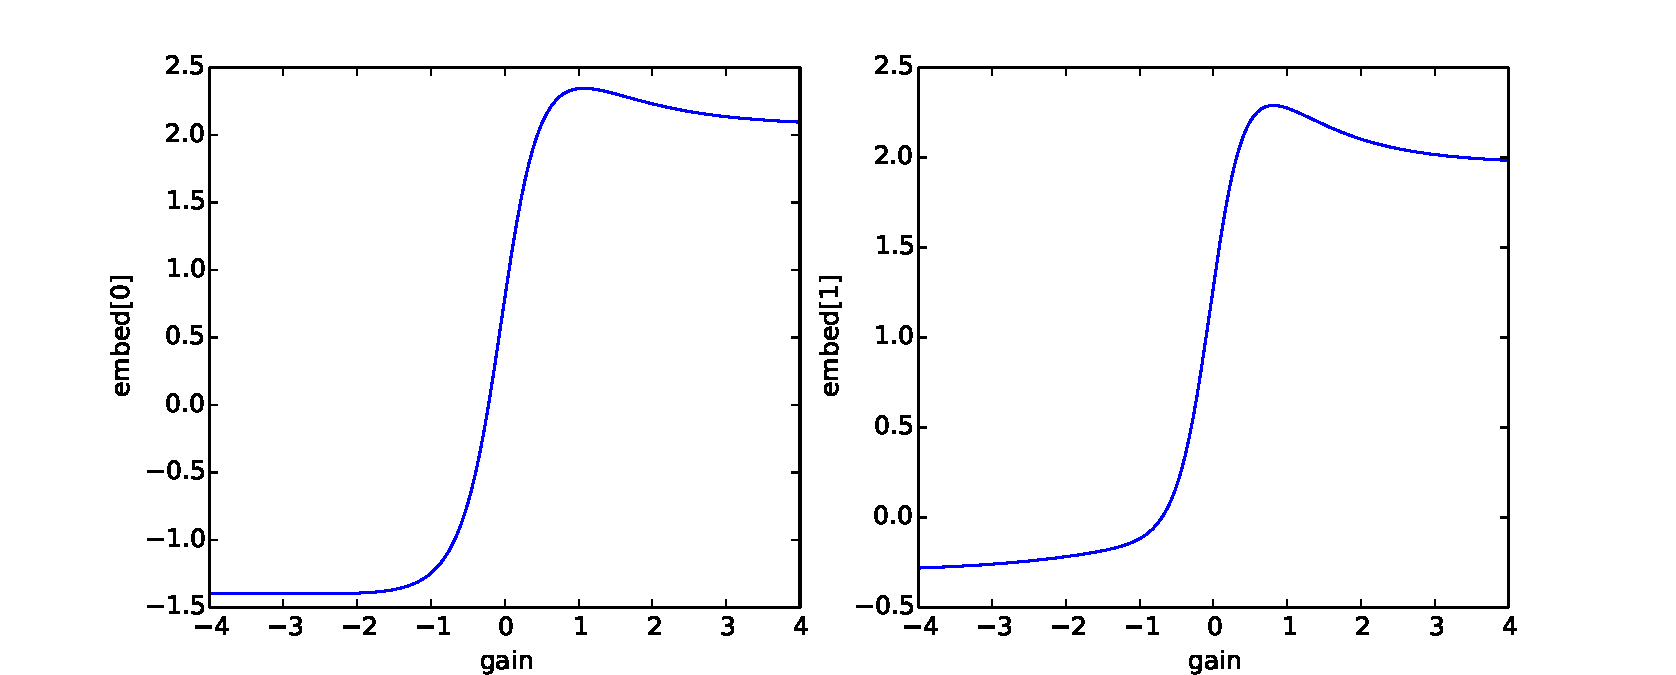
\includegraphics[trim={13.7cm 0 2cm 0}, clip, width=0.35\textwidth]{pointmass_embed_mapping.pdf}
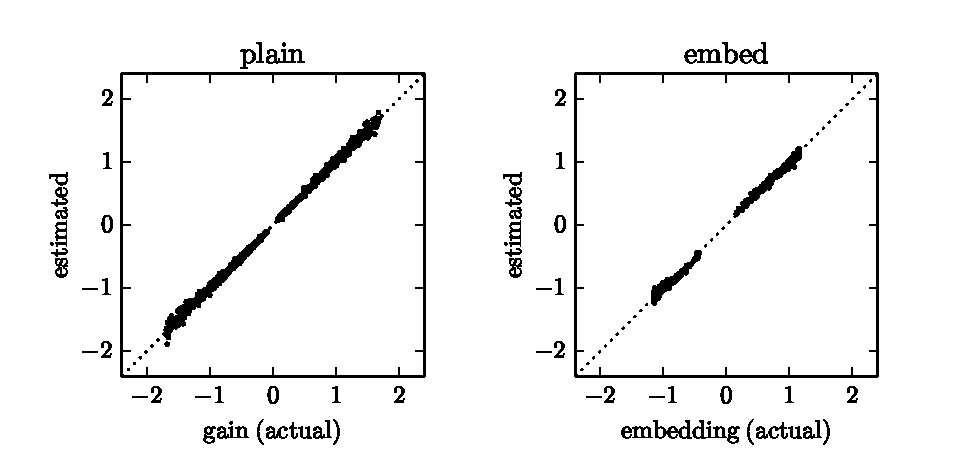
\includegraphics[trim={0.5cm 0 1cm 0}, clip, width=0.63\textwidth]{pointmass_embed_scatter.pdf}
\caption{
\emph{Left}: One dimension of learned mapping $\embedfn$ from gain factor $g$ to 2D embedding space $\latset$ in point-mass environment.
\emph{Middle}: Actual vs. estimated gain parameter $g$ for \plain{} policy.
\emph{Right:} Actual vs. estimated learned embedding in $\latset$ with \embed{} policy (one of two dimensions).
Embedding spreads positive and negative gain to more distant clusters.
}
\label{embed-mapping}
\end{figure}


\figref{embed-mapping} illustrates the learned mapping from the gain factor $g$
to the embedding space $\latset$.
The scatter plots compare the ground truth embedding values
against those estimated by $\idfn$ in the \embed{} policy,
and the ground truth gain factor $g$ against the values estimated by the equivalent of $\idfn$ in the \plain{} policy.
%Against the $x-$axis, density estimates are shown.
Both illustrate that the learned embedding function $\embedfn$ ``squashes'' the gain factor $g$ into positive and negative clusters.
The separation between these clusters is magnified, making it easier for the policy to switch between two disjoint behavior styles depending on the sign of the gain factor.
The ``squashing'' does not impede the task reward of the policy,
since an identical bang-bang control policy is optimal for any magnitude of $g$ -- only the sign of the input needs to change.

Figure~\ref{fig:conditional_action} shows the policy output $\pi_\latvar(a|\idvar)$ conditioned on
the gain factor $g$ at the initial task state $s_{t0} = (1, 1)$.
This illustrates that the policy contains two disjoint behaviors,
and switches between these behaviors rapidly and precisely with the sign of the gain $g$.



\begin{figure}
\centering
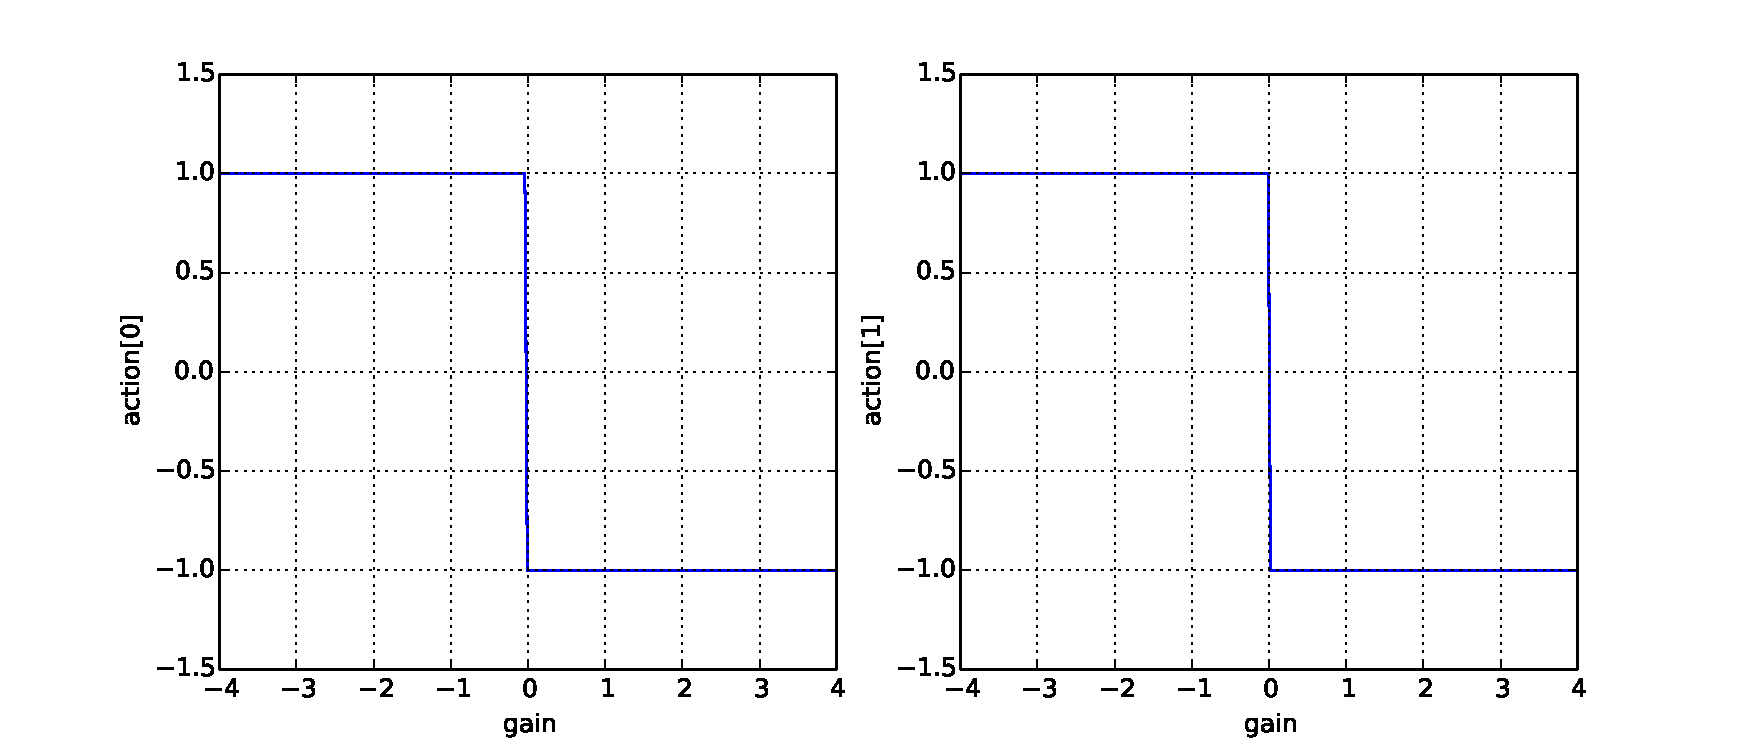
\includegraphics[width=0.85 \textwidth]{pointmass_conditional_action.pdf}
\caption{
Action of trained \embed{} policy at initial state (position $ = (1,1)$, velocity $=(0,0)$) conditioned on gain factor $g$.
Outputs are clipped to valid action range.
Plots show that policy has learned the optimal bang-bang control policy in both positive and negative gain scenarios.
\TODO{condense into fig. 2.}
}
\label{fig:conditional_action}
\end{figure}

\subsubsection{Disentangling of redundant features}

\begin{figure}
\centering
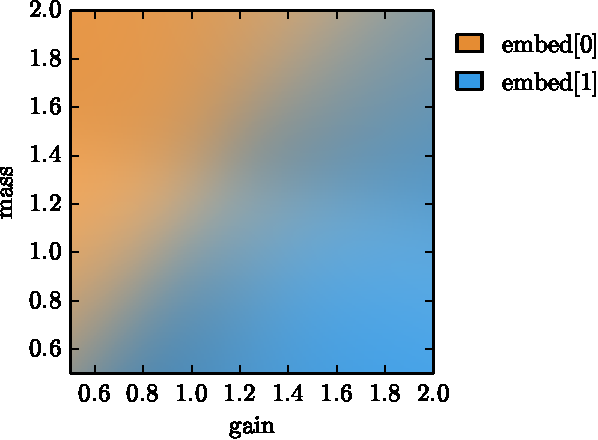
\includegraphics[width=0.5\textwidth]{embed_colors.pdf}
\caption{
Heatmap-style plot of learned embedding space disentanging redundant \sysid{} parameters.
Graph axes represent true dynamics parameters; each color represents one dimension of the learned 2D embedding.
In point-mass environment with parameters of gain $g$ and mass $m$,
the dynamics only depend on the $g/m$ ratio.
The learned embedding reflects this; for example, the $g=m$ line is all mapped to similar embedding values.
Plot restricted to positive gain domain for clarity.
}
\label{fig:embed_colors}
\end{figure}
A primary benefit of our approach is its ability to distill potentially complex sets of dynamics parameters
into a simplified space where only the information needed to achieve good rewards is preserved.
We illustrate this by constructing a version of the point-mass environment with redundant features:
we add a mass parameter $m$ alongside the gain parameter $g$.
Now, the true acceleration of the point is proportional to $g/m$,
making all $(g, m)$ combinations with the same ratio indistinguishable to system identification.
This poses a problem for the \plain{} 
%or \extra{} frameworks
framework
because the learning problem of recovering the true $(g, m)$ from a state-action trajectory is ill-posed.
In contrast, our framework learns an embedding where all $(g, m)$ combinations with similar ratios are mapped to similar embedding values.
This embedding is visualized in Figure~\ref{fig:embed_colors}.

\begin{comment}
\begin{figure}
\centering
\TODO{learning curves for redundant point-mass.}
\caption{
Example of incompatibility between our observability objective \TODO{ref}
and attempting to reconstruct the true dynamics parameters
in redundant point-mass environment.
When $\alpha = 0.1$, \extra{} network alters its behavior in pursuit of the observability reward, but the dynamics parameters are impossible to identify.
The learning process is disturbed.
When $\alpha = 0$, \extra{} network does not alter its behavior
and learns a policy that accounts for the many-to-many characteristic of the system identification problem.
}
\label{fig:redundant_fail}
\end{figure}
\end{comment}


Note that the learned embedding in these examples is two-dimensional -- 
the human operator does not need to know the minimal dimensionality of the parameters after redundancies are removed.
This is important in scenarios with many parameters where identifying redundant parameters 
is not as simple as in the point-mass environment.

\subsection{Half-Cheetah Environment}

\begin{figure}[ht]
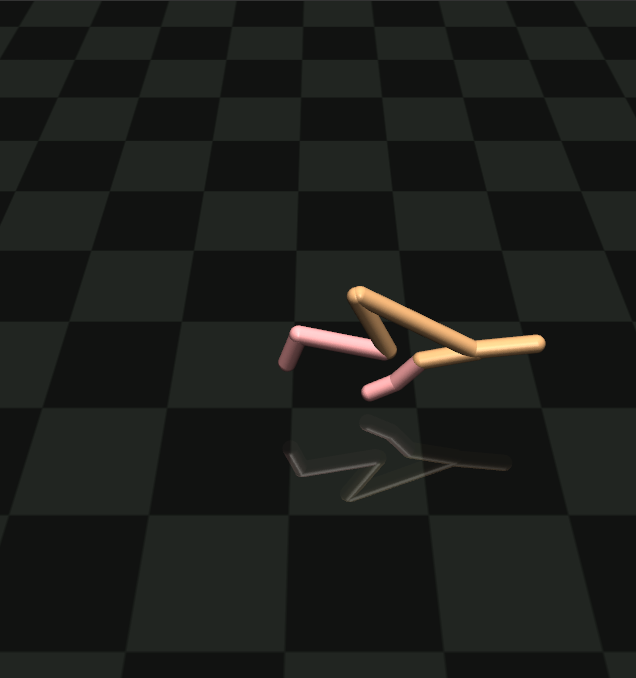
\includegraphics[trim=4cm 3cm 0cm 4cm, clip, width=0.22\textwidth]{cheetah_short.png}\hfill
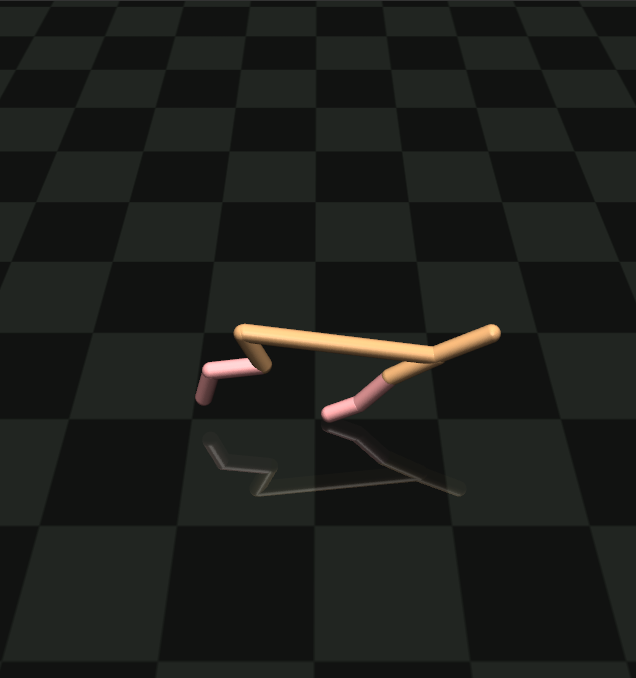
\includegraphics[trim=4cm 3cm 0cm 4cm, clip, width=0.22\textwidth]{cheetah_medium.png}\hfill
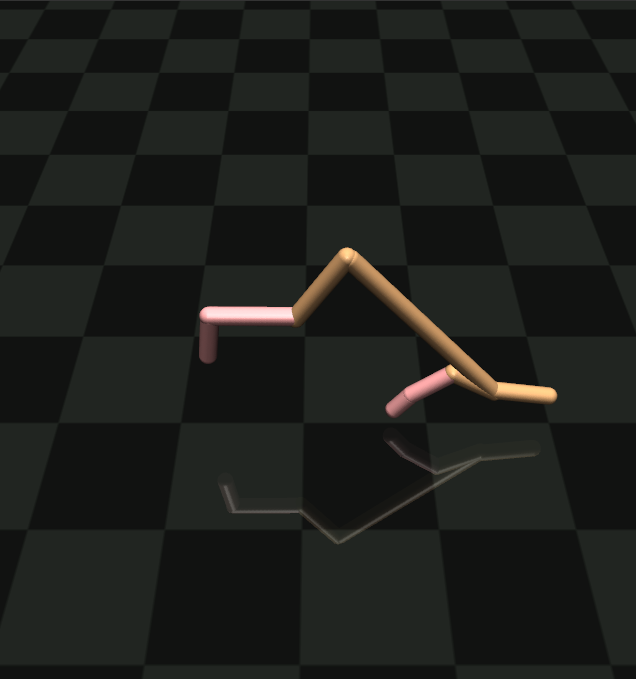
\includegraphics[trim=4cm 3cm 0cm 4cm, clip, width=0.22\textwidth]{cheetah_backleg.png}\hfill
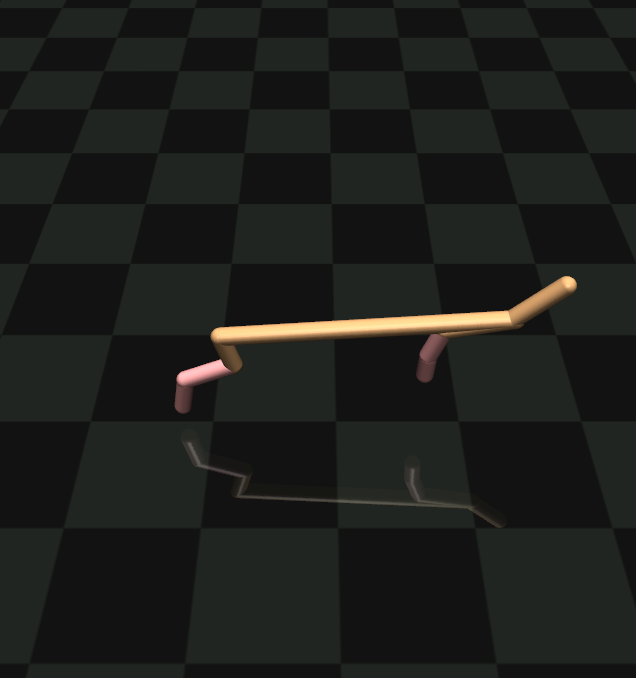
\includegraphics[trim=4cm 3cm 0cm 4cm, clip, width=0.22\textwidth]{cheetah_long.png}
\caption{Variations of Half-Cheetah environment produced by randomization of kinematic and dynamic properties.}
\label{cheetahs}
\end{figure}

As an example of a more complex task, we demonstrate results on the \emph{Half-Cheetah}
planar locomotion environment from the OpenAI Gym~\citep{openai-gym}.
The following parameters are randomized:
lengths of seven kinematic links,
damping, stiffness, and ranges of six planar revolute joints,
and gear ratios of six rotary actuators.
In total, 37 parameters are randomized.
The embedding space $\latset$ is chosen to be 8-dimensional.
Each end of the joint range is shifted by $\pm 0.3$ radians.
All other parameters are multiplied by a ratio log-uniformly distributed in the range $[\beta^{-1}, \beta]$ with $\beta = 1.75$.
\TODO{describe these perturbations more precisely}

Due to the architecture of the MuJoCo physics simulator used in this environment~\citep{todorov-mujoco},
it is not practical to sample new random dynamics parameters $\idvar$ for each training iteration.
Instead, we train on a fixed set of 256 randomized models.
At test time, we sample a new, independent set of 256 randomized models.
%Instead, we construct a ``universe'' of 256 models initially, and randomly choose 8 of these environments for each training iteration.
%At test time, we resample a new ``universe'' of models.

Results from these experiments are shown in Table~\ref{cheetah}.
The data show that, while the \plain{} policy performs slightly better in training,
it suffers from worse generalization error.
The \embed{} policies achieves lower generalization error and higher test rewards.
Note that the training, as well as the test, performance for nonzero $\alpha$
is better for both \embed{} and \plain{} policies.
We hypothesize that behaving the same for all $\idvar$ values, like the \blind{} policy,
is a local optimum in the policy space,
whereas the optimal policy specializes for each $\idvar$,
but this optimum is more difficult to find.
The observability reward provides an additional incentive
for the policy to behave differently for environments with different $\idvar$ values,
pulling it away from the undesirable local optimum.

\subsubsection{Insensitivity to dimensionality of $\latset$}
Our approach introduces a new hyperparameter: the dimensionality of $\latset$.
In this experiment, we show that our approach is not overly sensitive to this choice.
\TODO{This experiment.}

\TODO{Conclusion of experimental section.}
%In summary, the experimental results in this section suggest that learning the embedding space $\latset$
%is beneficial both for the training process and for the test performance.

\section{Conclusion}
In this paper, we demonstrated a novel framework for training robot control policies
that can adapt online in real time to variations in system dynamics parameters.
We learn an embedding space that distills the full system identification information
and can disentangle redundant and unobservable parameters, while preserving the information that is useful for decision making.
We introduce an observability reward function in the reinforcement learning reward,
such that the control policy is encouraged to behave in a way that makes system identification easier.
Experimental results illustrate the desirable properties of the embedding space on a low-dimensional problem
and demonstrate improved training performance and test generalization compared to baselines
where the embedding space and observability reward are not used.
Future work will focus on applying this method to simulation-to-reality transfer on a real robot.
We also expect to see a greater benefit from the embedding space on more complex systems with very large system identification spaces.

\clearpage
%\acknowledgments{}
\bibliography{bibliography}{}

\end{document}
